\documentclass[14pt, a4paper]{article}
\usepackage[T2A]{fontenc}
\usepackage[utf8]{inputenc}
\usepackage[russian]{babel}
\usepackage[left=3cm, right=1.5cm, top=2cm, bottom=2cm]{geometry}
\usepackage{indentfirst}
\usepackage{microtype}
\usepackage{array}
\usepackage{xcolor}
% \usepackage{times}
\usepackage{tempora}
\usepackage{ulem}
\usepackage{setspace}
\usepackage{amsmath}
\usepackage{booktabs}
\usepackage{graphicx}
\usepackage{float}
\usepackage{listings}
\graphicspath{{reports/figures/}{figures/}}
\lstset{basicstyle=\ttfamily\small, breaklines=true, columns=fullflexible, frame=single, keepspaces=true}
\pagestyle{empty}

\makeatletter
\renewcommand\section{\@startsection {section}{1}{\parindent}%
  {-3.5ex \@plus -1ex \@minus -.2ex}%
  {0.5ex}%
  {\normalfont\Large\bfseries}}
\renewcommand\tableofcontents{%
  \begin{center}\Large\bfseries\contentsname\end{center}%
  \@starttoc{toc}%
}
\renewcommand*\l@section{\@dottedtocline{1}{0em}{1.5em}}
\makeatother

\begin{document}
\onehalfspacing

\begin{center}
    \textbf{ФЕДЕРАЛЬНОЕ ГОСУДАРСТВЕННОЕ АВТОНОМНОЕ ОБРАЗОВАТЕЛЬНОЕ} \\
    \textbf{УЧРЕЖДЕНИЕ ВЫСШЕГО ОБРАЗОВАНИЯ} \\
    \textbf{«МОСКОВСКИЙ АВИАЦИОННЫЙ ИНСТИТУТ} \\
    \textbf{(НАЦИОНАЛЬНЫЙ ИССЛЕДОВАТЕЛЬСКИЙ УНИВЕРСИТЕТ)»}
\end{center}

\begin{center}
    \bfseries Институт №8 «Компьютерные науки и \\
    \bfseries прикладная математика» \\
    \bfseries Кафедра 806 «Вычислительная математика \\
    \bfseries и программирование»
\end{center}

\vspace{3cm}

\begin{center}
    \Large\bfseries Отчет \\
    \vspace{0.5cm}
    \mdseries по лабораторной работе №3.3
\end{center}

\vfill

\noindent
\hfill
\begin{tabular}{ll}
Группа:       & М8О-307Б-21 \\
Студент:      & М. С. Ивченко \\
Преподаватель:& доц. В. В. Киндинова \\
Оценка:       & \underline{\makebox[3cm][c]{}} \\ [0.2cm]
Дата:         & \underline{\makebox[3cm][c]{}}
\end{tabular}

\vfill

\begin{center}
    Москва \\
    2026
\end{center}

\newpage

\setcounter{tocdepth}{2}
\tableofcontents
\newpage

\section*{Тема}
\addcontentsline{toc}{section}{Тема}
Цель данной лабораторной работы -- изучить приближение таблично заданных данных в ситуации, когда точное прохождение через все точки не является главным требованием. Метод наименьших квадратов позволяет построить простую аппроксимирующую зависимость и оценить суммарную ошибку приближения.

\section*{Задание}
\addcontentsline{toc}{section}{Задание}
Для таблично заданной функции путем решения нормальной системы МНК найти приближающие многочлены а) 1-ой и б) 2-ой степени. Для каждого из приближающих многочленов вычислить сумму квадратов ошибок. Построить графики приближаемой функции и приближающих многочленов.

\section*{Теория}
\addcontentsline{toc}{section}{Теория}
Метод наименьших квадратов используется для аппроксимации, когда не требуется проходить точно через все табличные точки. Вместо интерполяции строится функция, которая в среднем находится как можно ближе к данным. Для многочлена
\[
    P_m(x)=c_0+c_1x+\ldots+c_mx^m
\]
нужно подобрать коэффициенты $c_j$, минимизирующие сумму квадратов отклонений
\[
    S=\sum_{i=0}^n (P_m(x_i)-y_i)^2.
\]
Квадраты используются потому, что положительные и отрицательные ошибки не компенсируют друг друга, а сама функция $S$ становится дифференцируемой по коэффициентам.

Если записать значения многочлена в матричном виде, получим $Xc\approx y$, где строки матрицы $X$ имеют вид $(1,x_i,x_i^2,\ldots,x_i^m)$. Условие минимума $\partial S/\partial c_j=0$ приводит к нормальной системе
\[
    (X^TX)c=X^Ty,
\]
где $X$ -- матрица признаков. Решение этой системы дает коэффициенты многочлена наилучшего среднеквадратичного приближения.

Для сравнения разных степеней аппроксимации вычисляется остаточная сумма квадратов
\[
    S_m=\sum_{i=0}^n(P_m(x_i)-y_i)^2.
\]
Обычно при увеличении степени $S_m$ уменьшается, но слишком высокая степень может привести к переобучению и колебаниям. В лабораторной работе сравниваются многочлены первой и второй степени: линейная модель показывает общий тренд, квадратичная дополнительно учитывает кривизну данных.

\begin{lstlisting}[language=Python]
feature_matrix = np.vander(x, N=degree + 1, increasing=True)
normal_matrix = feature_matrix.T.dot(feature_matrix)
right_side = feature_matrix.T.dot(y)
coefficients = solve_system(p, L, U, right_side)
\end{lstlisting}

\section*{Ход лабораторной работы}
\addcontentsline{toc}{section}{Ход лабораторной работы}
Использовалась таблица
\[
\begin{array}{c|rrrrrr}
x_i&-5&-3&-1&1&3&5\\\hline
y_i&2.9442&2.8198&2.3562&0.7854&0.32175&0.1974
\end{array}
\]
Найдены приближающие многочлены:
\[
P_1(x)=-0.3256992857x+1.5707916667,
\]
\[
P_2(x)=0.0000002232x^2-0.3256992857x+1.5707890625.
\]
Сумма квадратов ошибок для обоих вариантов практически одинакова: $S_1\approx S_2\approx0.7006866120$. Дополнительно построенный кубический многочлен дал $S_3=0.1411740353$, что показывает влияние добавления нечетного кубического члена.

\begin{figure}[H]
    \centering
    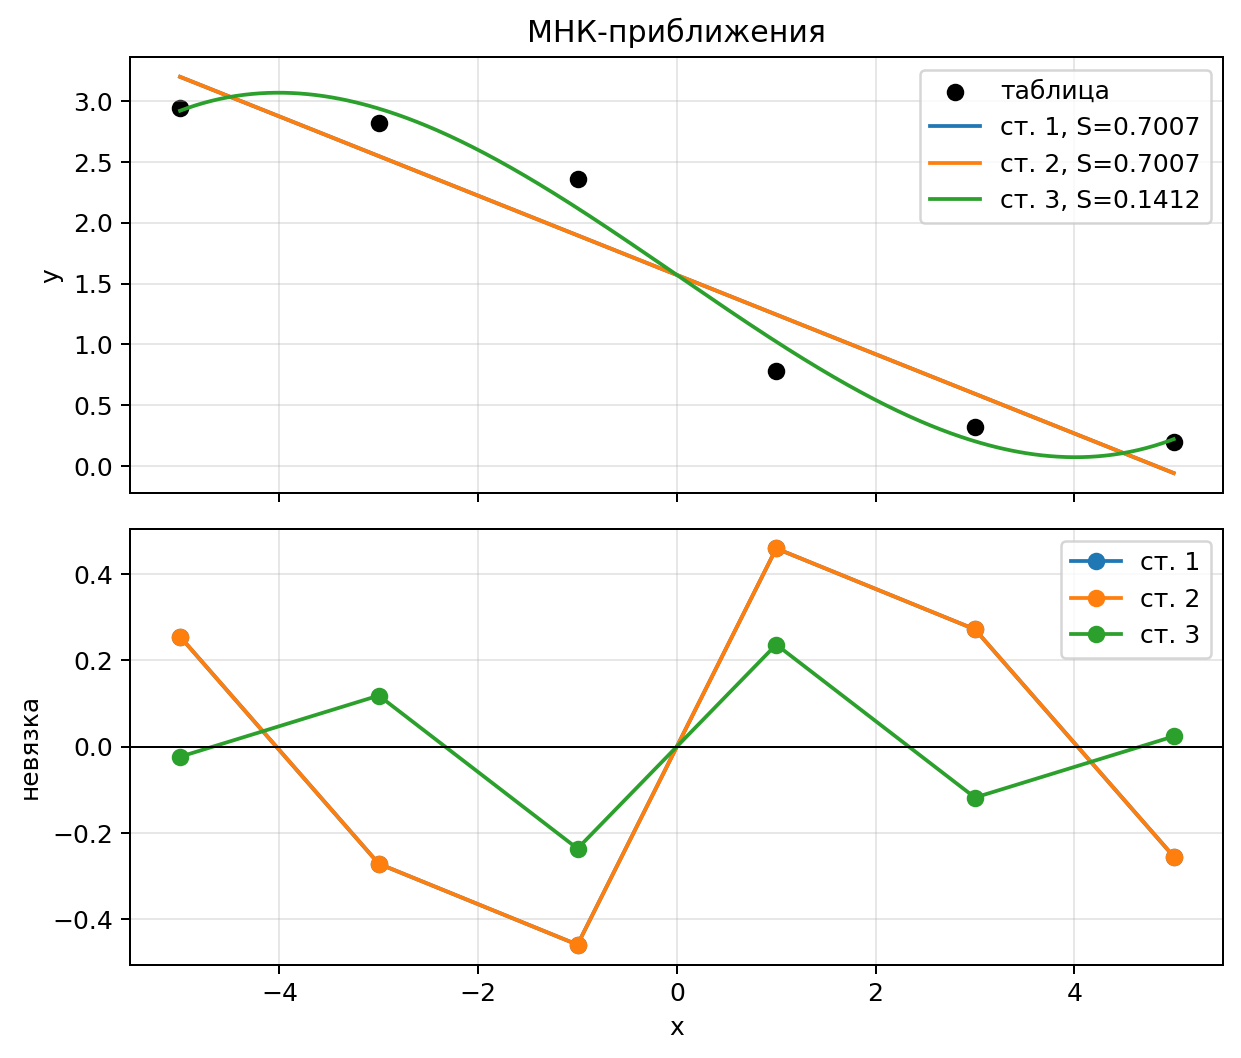
\includegraphics[width=0.86\textwidth]{lab3_3_least_squares.png}
    \caption{МНК-приближения и невязки для многочленов степеней 1, 2 и 3.}
\end{figure}

\section*{Выводы}
\addcontentsline{toc}{section}{Выводы}
Многочлены первой и второй степени почти совпали, так как коэффициент при $x^2$ оказался близок к нулю. Это отражает почти симметричную структуру данных варианта; повышение степени до трех заметно уменьшает сумму квадратов ошибок.

\end{document}
